
        \documentclass{exam-zh}
        \usepackage{siunitx}
        \examsetup{
          page/size=a4paper,
          paren/show-paren=true,
          paren/show-answer=false,
          fillin/show-answer=false,
          solution/show-solution=false
        }
        \ExamPrintAnswerSet{
          sealline/show=true,
          page/size=a3paper,
          paren/show-answer=false,
          fillin/show-answer=false,
          solution/show-solution=false,
        }
        \everymath{\displaystyle}
        \title{路丁康 2024-05-05}\subject{几何 相似/全等三角形}
        \begin{document}
        \maketitle
        
        \begin{problem}
        等腰三角形,腰上的高线长度是腰长的一半,求等腰三角形顶角的角度
        \end{problem}
        
        \begin{problem}
        如图,在平行四边形$ABCD$中,$BD$平分角$\angle ABC$。
        \begin{enumerate}
        \item 求证:平行四边形$ABCD$是菱形
        \item 连接$AC$交$BD$于点$O$,延长$BC$到点$E$,在$\angle DCE$的内部做射线$CM$,使得角$\angle ECM=15^\circ$,过点$D$做$DF\perp CM$于点$F$。若$\angle ABC=70^\circ$,$DF=\sqrt{5}$,求$\angle ACD$的度数及$BD$的长
        \end{enumerate}
        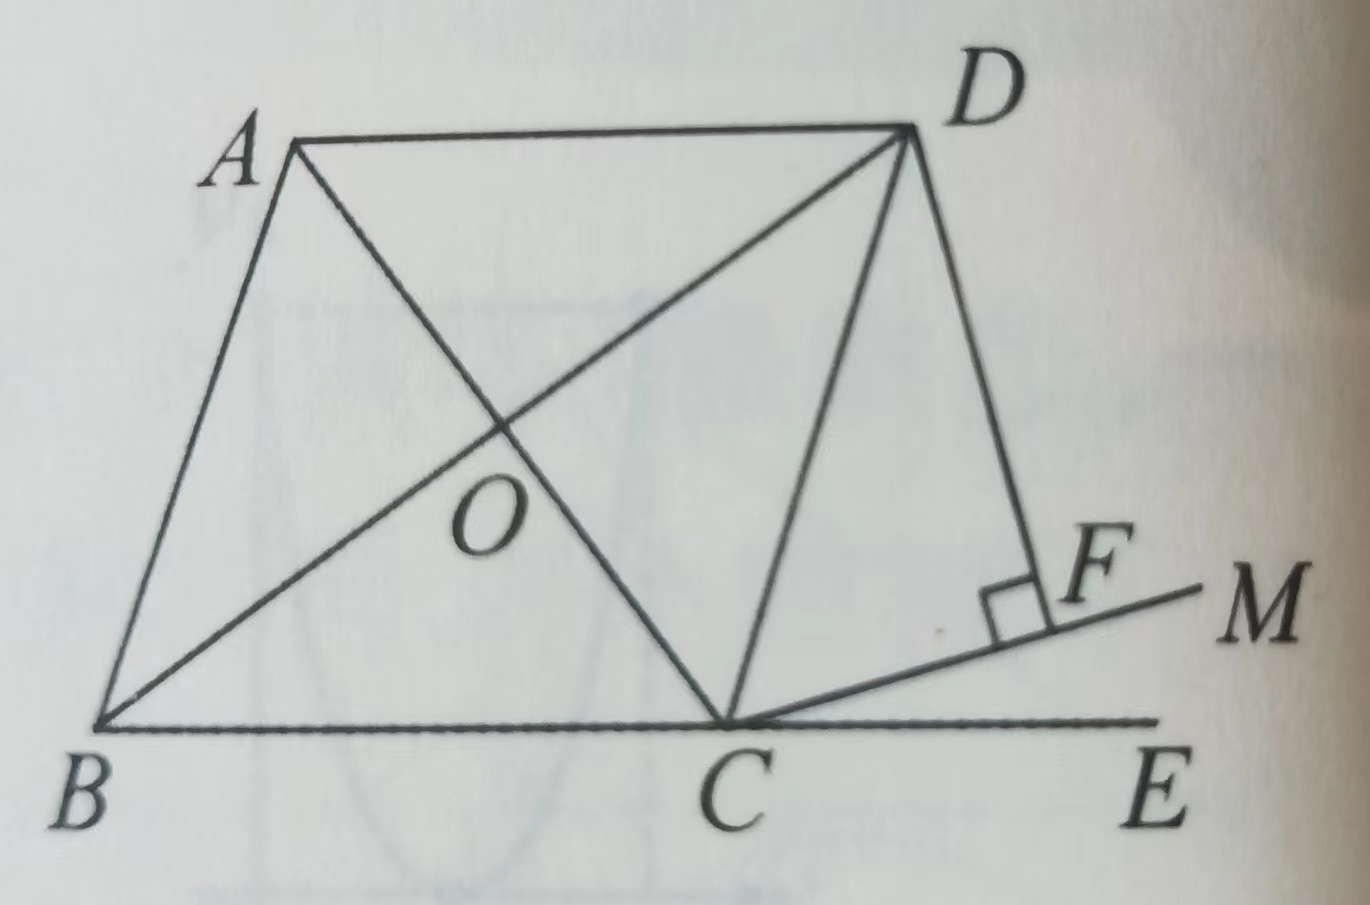
\includegraphics[width=5cm]{p1.jpg}
        \end{problem}
        
        \end{document} 